\documentclass[10pt]{beamer}
\usetheme{Malmoe}
\colorlet{beamer@blendedblue}{green!40!black}
\setbeamertemplate{navigation symbols}{}
\newcommand*\oldmacro{}%
\let\oldmacro\insertshorttitle%
\renewcommand*\insertshorttitle{%
\oldmacro\hfill%
\insertframenumber\,/\,\inserttotalframenumber}

\usepackage{xfrac}
\usepackage{caption}
\usepackage{hyperref}
\usepackage[makeroom]{cancel}
\usepackage{ amssymb }
\usepackage{appendixnumberbeamer}
%\usepackage{tikz-feynman}
\usepackage{graphicx}
\begin{document}
\title{Searching for Ultra Rare Processes with the Large Hadron Collider}
\author[\hyperlink{supplemental}{J. Barkeloo}]{Jason Barkeloo}

\titlegraphic{
\includegraphics[width=4cm]{../ATLAS-Logo-Ref-RGB.png}\hspace*{2.75cm}~%
   
\includegraphics[width=4cm]{../uo_logo_green_on_white_2.jpg}
}

%\frame{\frametitle{}
%\begin{itemize}
%\item
%\end{itemize}
%}

\date{February 24, 2020}
\frame{\titlepage}
\frame{\frametitle{Overview}\tableofcontents[]}%hidesubsections]}
\section{The Large Hadron Collider and The Standard Model of Particle Physics}
%\frame{\frametitle{Table of Contents}\tableofcontents[currentsection,hideothersubsections]}
%%%%%%%%%%%%%%%%%%%%%%%%%%%%%%%%%%%%%%%%%%%%%%%%%%%%%%%%%

\subsection{LHC and ATLAS}

\frame{\frametitle{The Large Hadron Collider}
\centering
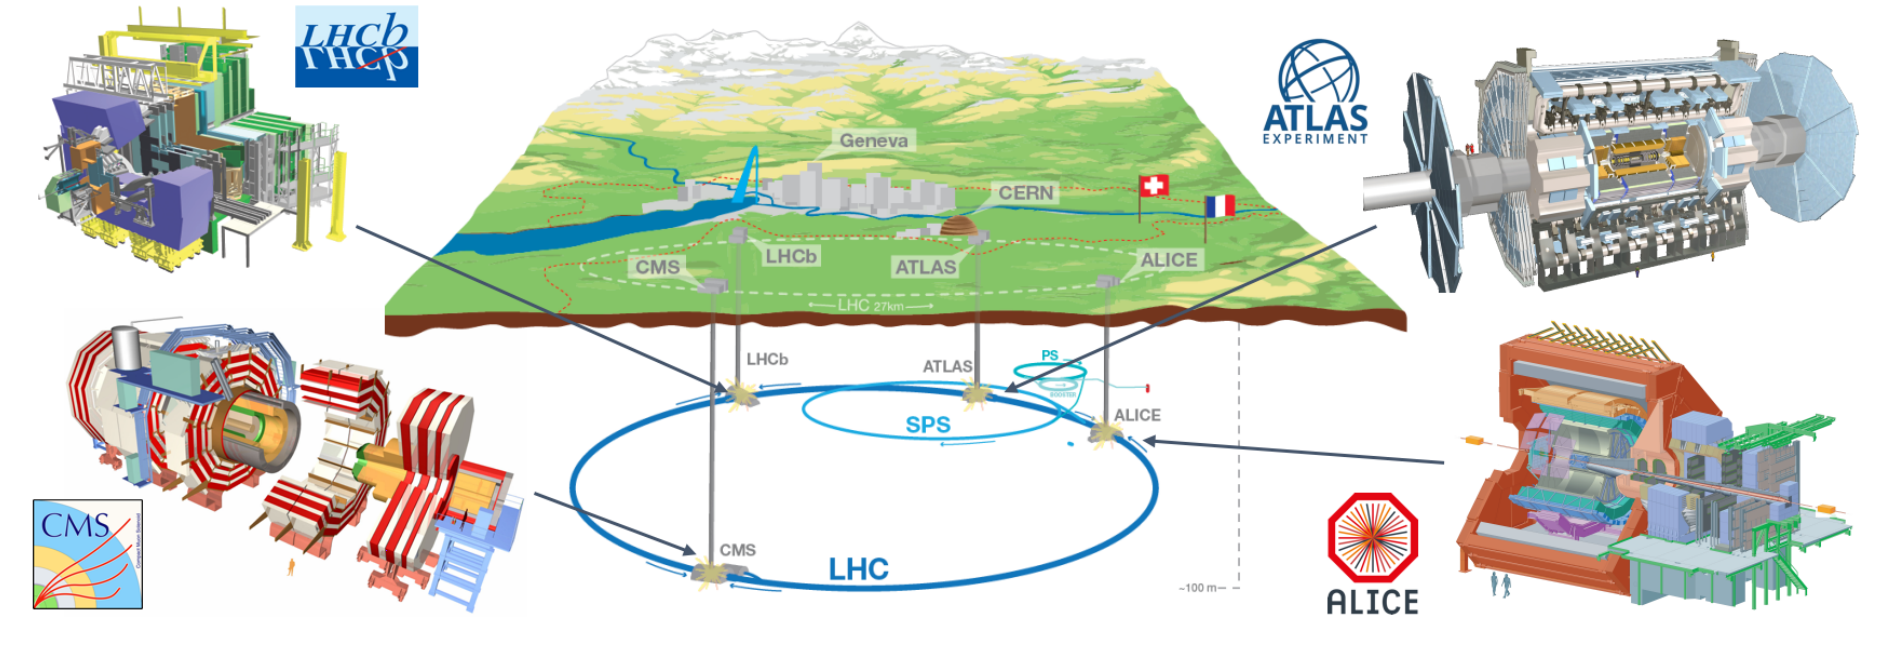
\includegraphics[width=\textwidth]{../../Thesis/ThesisImages/LHCImages/LHCDetecPlacement.png}
\begin{itemize}
\item 27km ring beneath Franco-Swiss border

\item Collides protons at center of mass energy 13TeV
\begin{itemize}
\item Proton Therapy Machines around 100MeV - 5 orders of magnitude smaller!
\end{itemize} %(compared to ~100MeV Proton Therapy Energies)
\item Over 10 Quadrillion ($10^{15}$) events produced within the ATLAS detector so far
\end{itemize}
}

\frame{\frametitle{The ATLAS Detector}
\centering
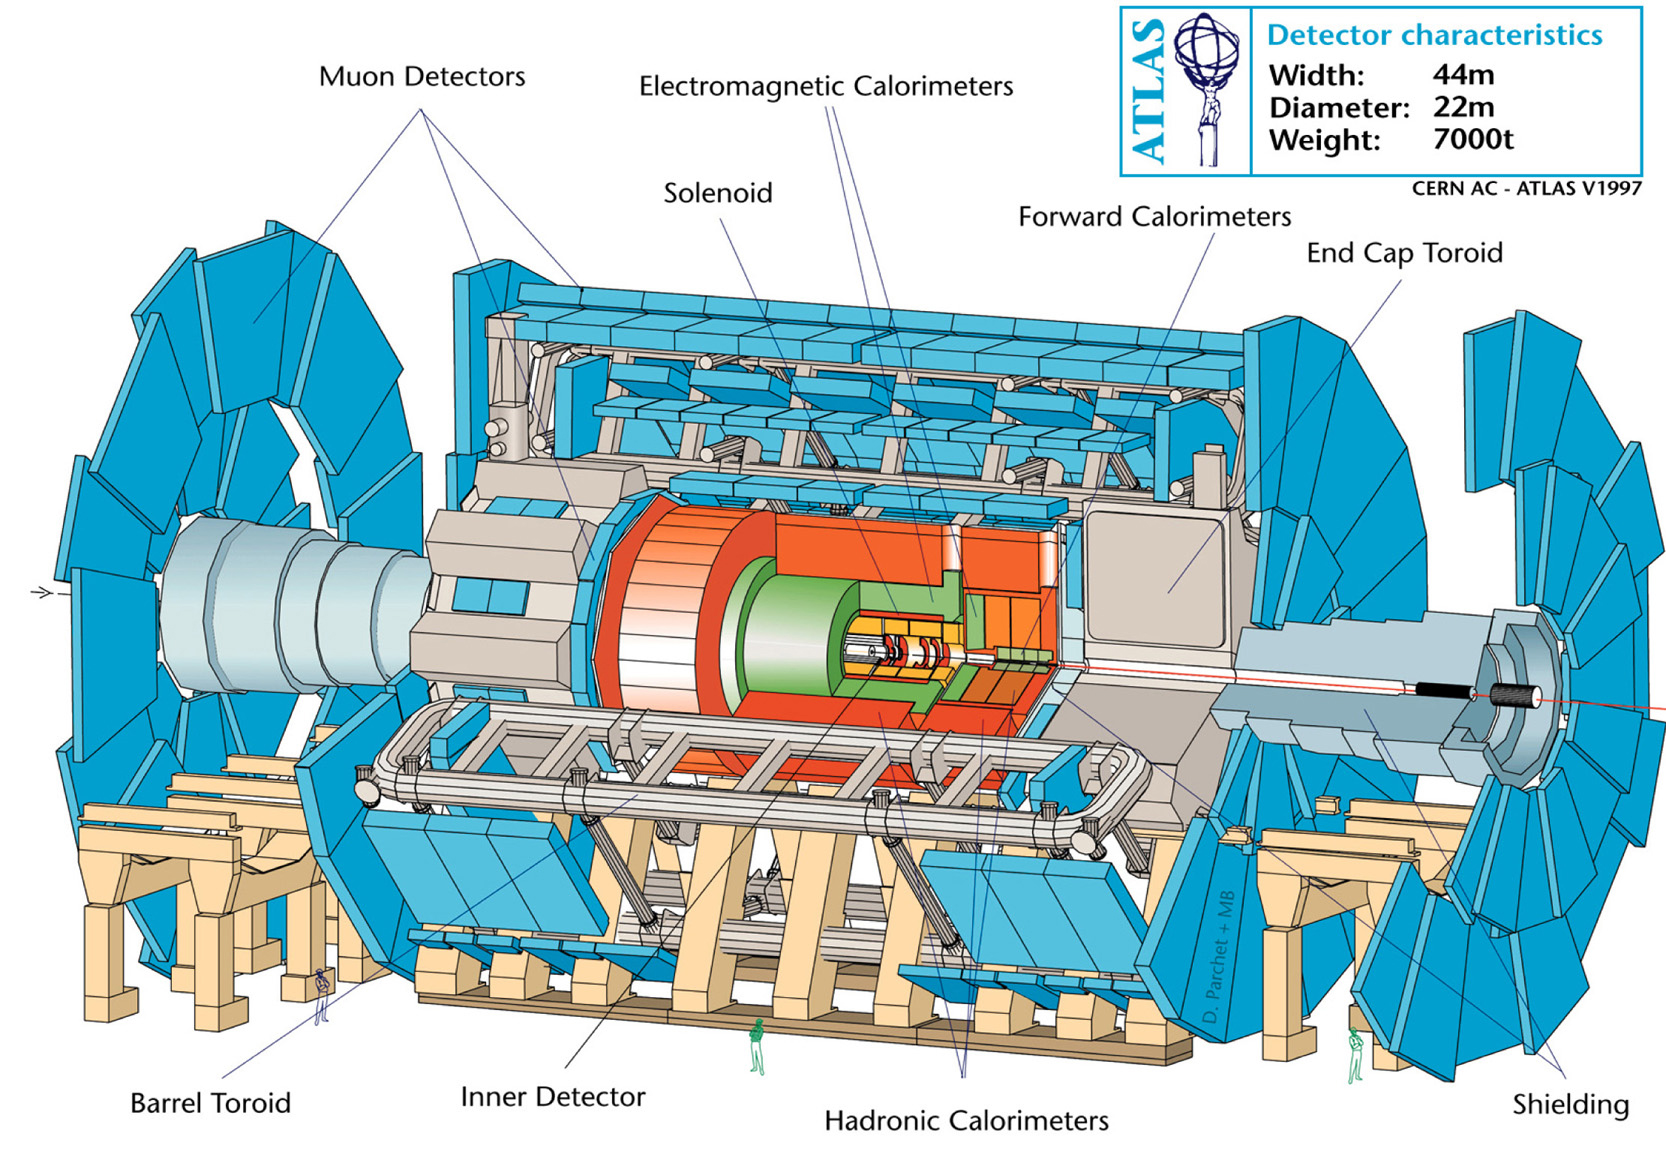
\includegraphics[width=.9\textwidth]{../../Thesis/ThesisImages/LHCImages/atlasdet.jpg}
}

\frame{\frametitle{Events in ATLAS}
\begin{columns}
\begin{column}{0.5\textwidth}
\centering
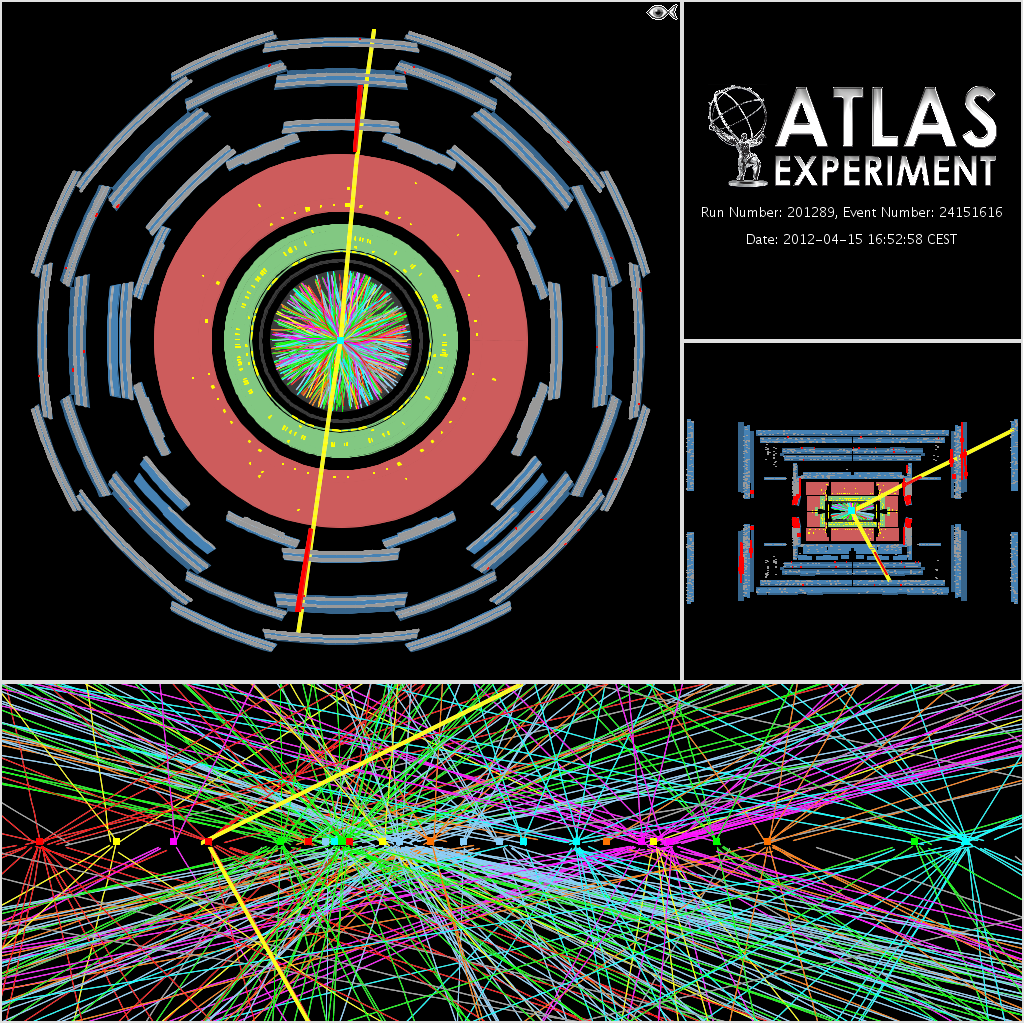
\includegraphics[width=\textwidth]{../../Thesis/ThesisImages/LHCImages/2012_highPileup.png}
\end{column}
\begin{column}{0.5\textwidth}
\begin{itemize}
\item LHC provides around 600 million interactions/second
\item Save compelling events $\rightarrow$ 10s of PB/year
\item Extremely large, messy data sets
\item Detector well modeled with \textsc{Geant4} 
\item Monte Carlo techniques used for background event generation
\end{itemize}
\end{column}
\end{columns}


}

\subsection{The Standard Model of Particle Physics}
\frame{\frametitle{The Standard Model of Particle Physics}
\centering
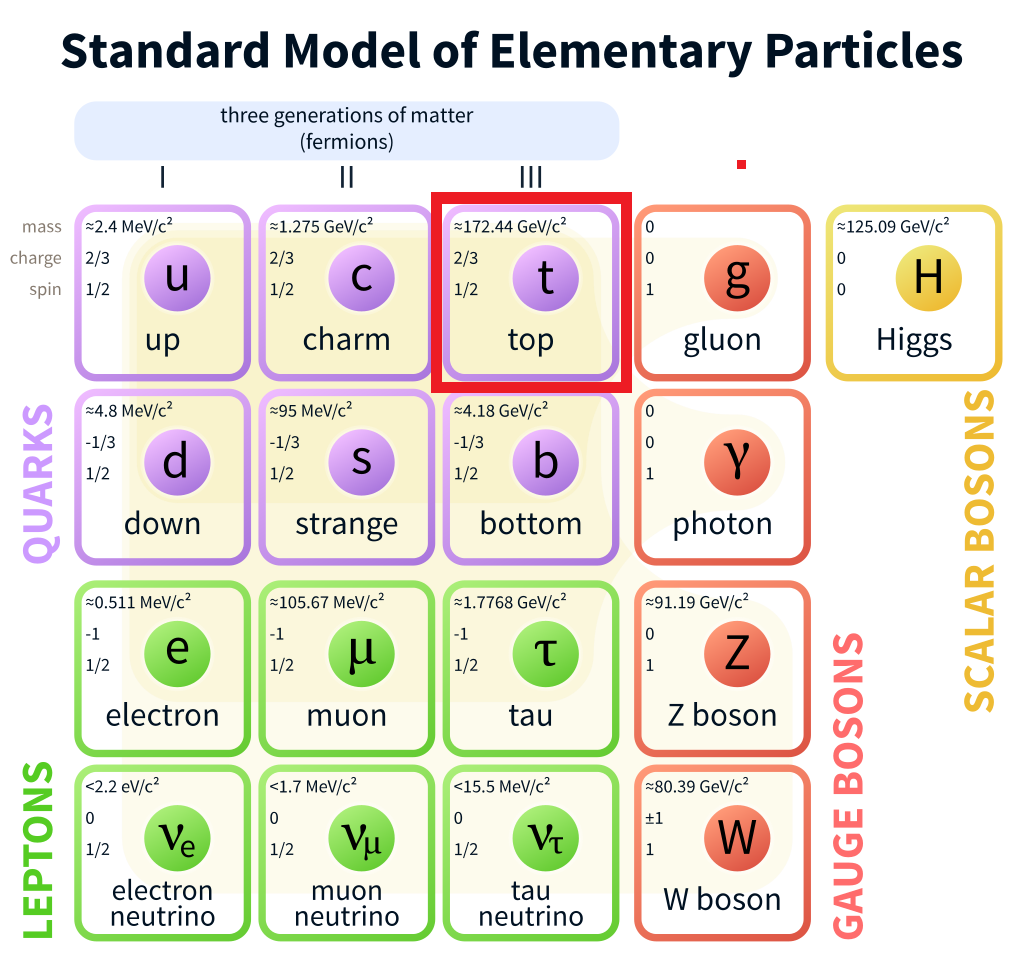
\includegraphics[width=.55\textwidth]{Images/SMParticles.png}
\begin{itemize}
\item Our current best theory that attempts to explain the building blocks of nature
	\begin{itemize}
	\item Experimentally precise and well behaved
	\item Very few exceptions (i.e., Dark Matter Abundance)
	\end{itemize}
	\vspace{\baselineskip}
\end{itemize}
}

\section{Search For Ultra Rare Decays}
\subsection{The Top Quark}
\frame{\frametitle{The Top Quark and Flavor Changing Neutral Currents}
\begin{columns}
\begin{column}{0.5\textwidth}
\begin{itemize}
\item Heaviest fundamental particle%, $172.5\text{GeV/c}^{2}$
\item Lifetime $5\times10^{-25}$s
\begin{itemize}
\item Allows study of single quark decay
\end{itemize}
\item Top decays to bW 100\% of the time
\item Expect $\approx 10^8$ top pair events
\end{itemize}
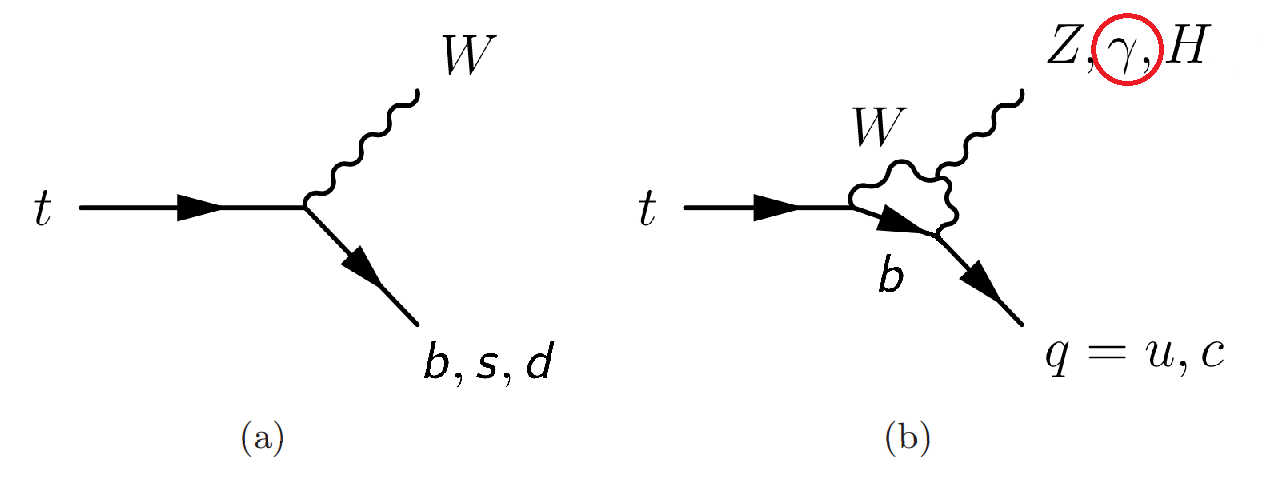
\includegraphics[width=\textwidth]{Images/SMTopDecays.png}
\end{column}
\begin{column}{0.5\textwidth}
\centering
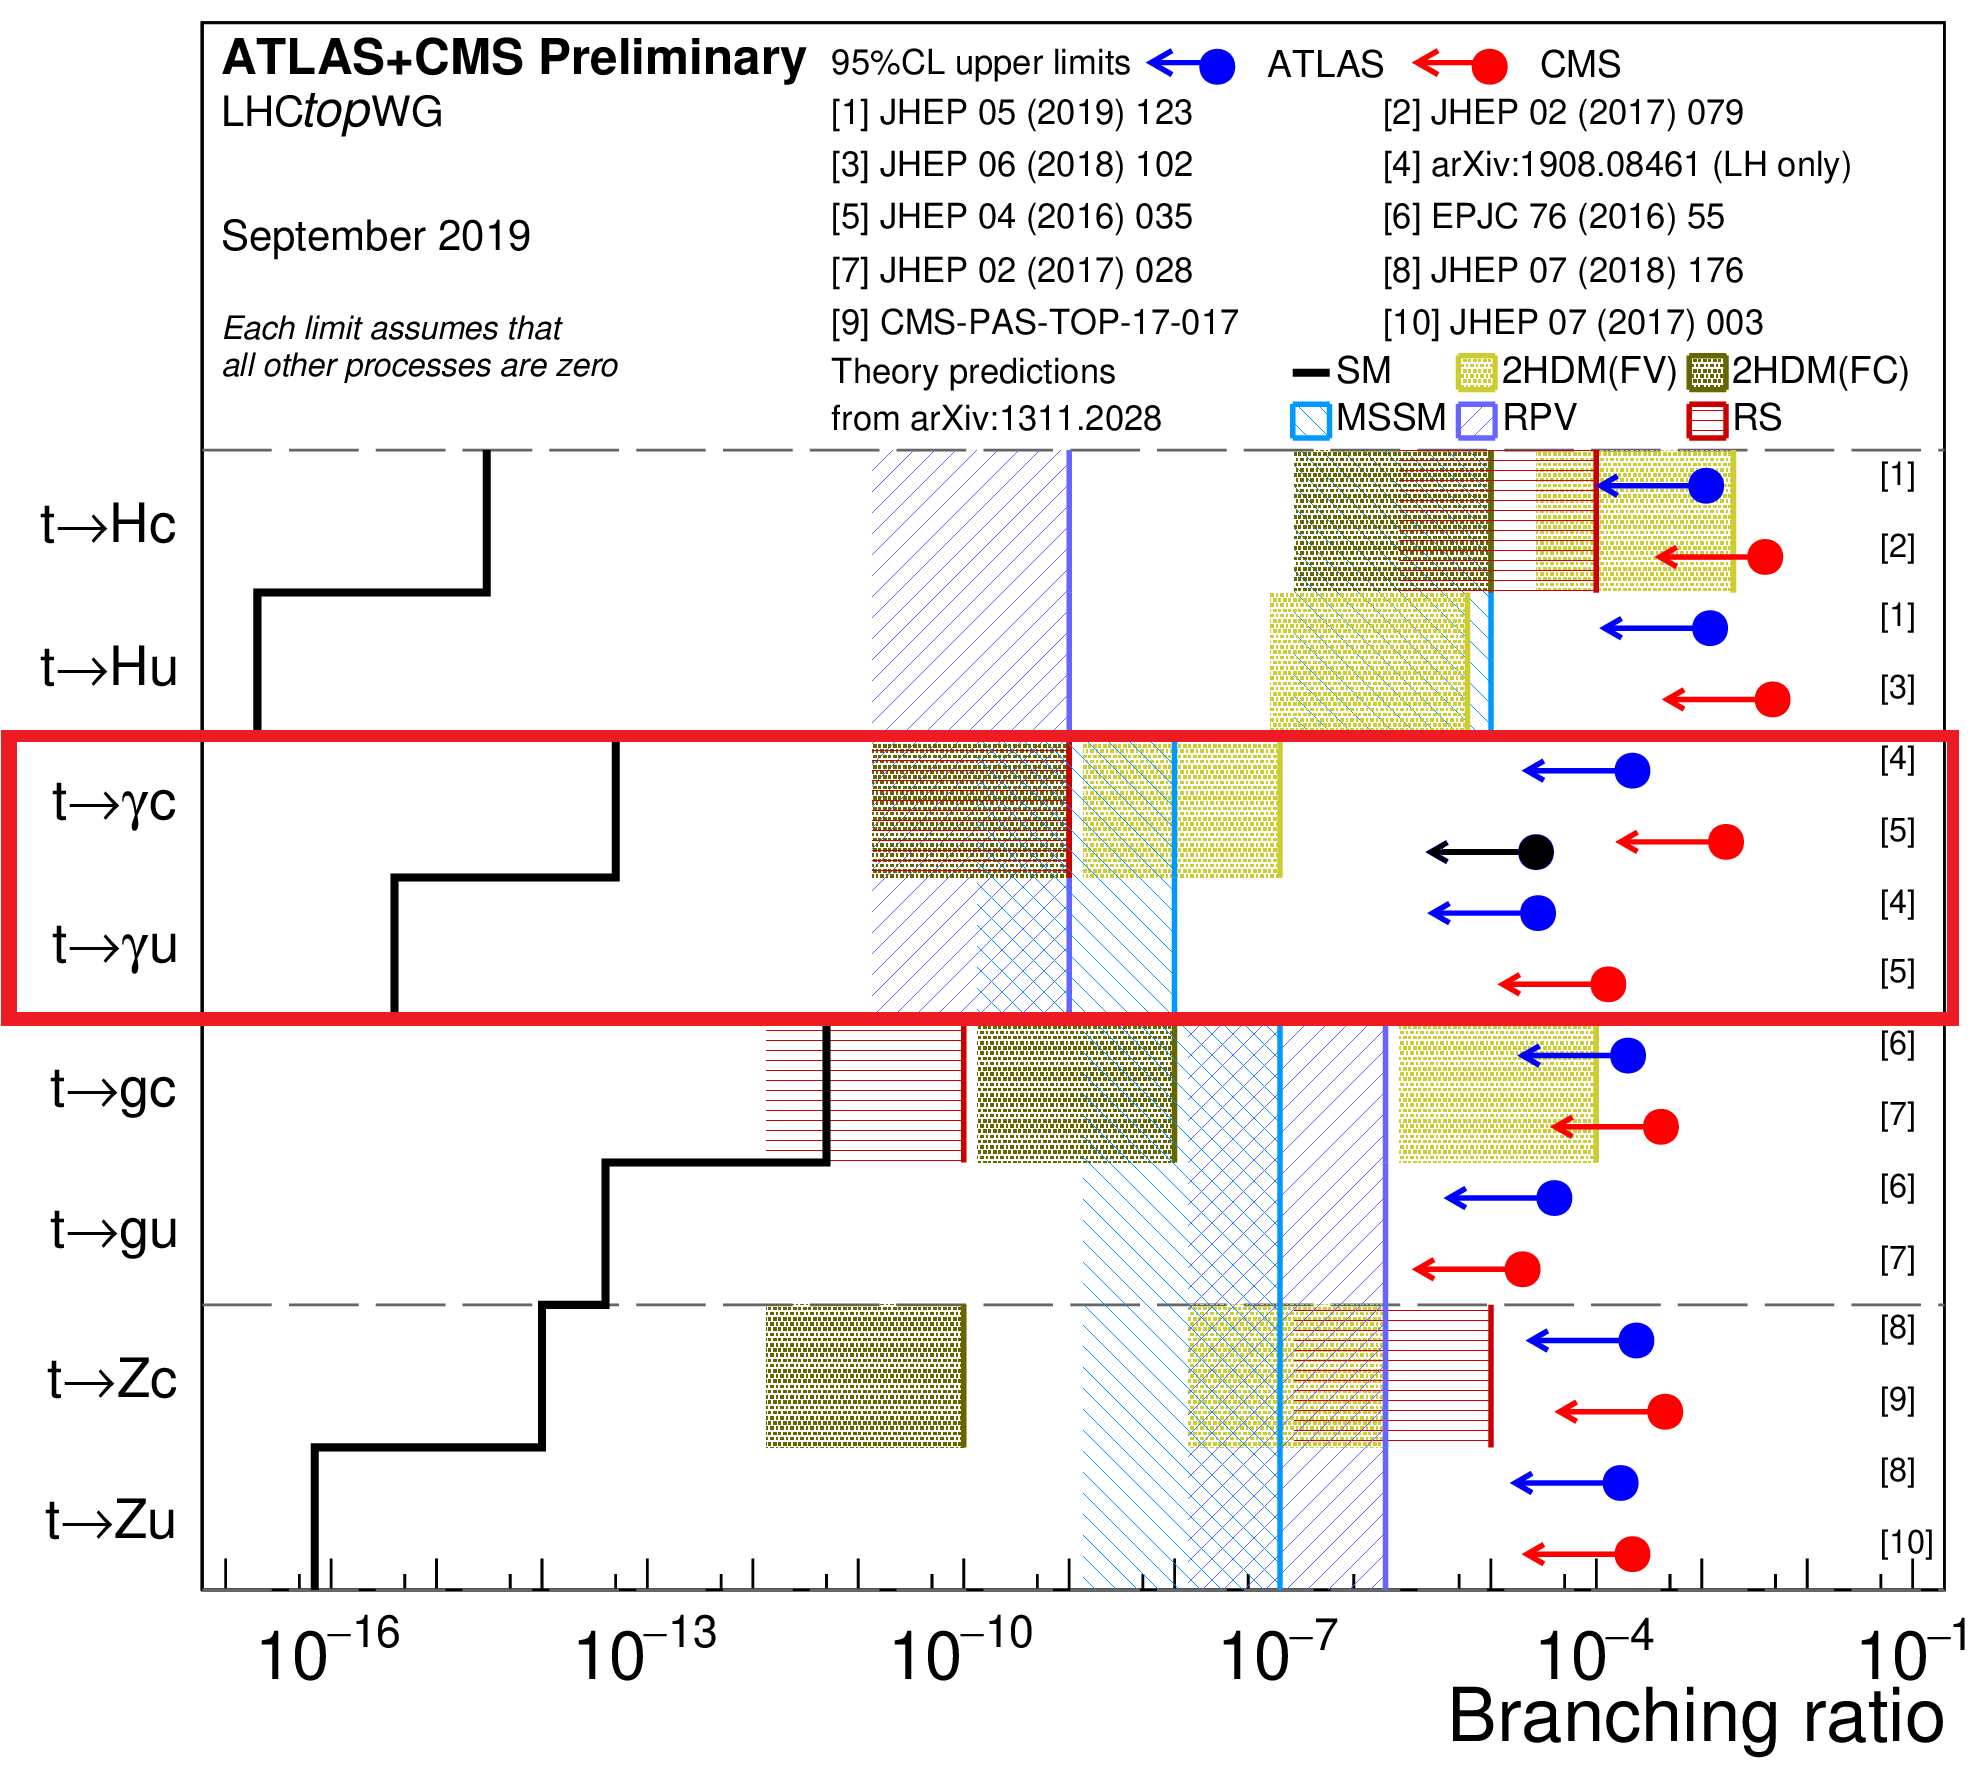
\includegraphics[width=\textwidth]{Images/AllFCNCLimits.png}
\end{column}
\end{columns}
}

\subsection{Machine Learning}
\frame{\frametitle{Neural Networks}
\begin{itemize}
\item Advanced pattern recognition used to classify events
\item A dense neural network is used with various low and high level variable inputs
\item Supervised learning used to approximate any multidimensional function
\end{itemize}
\centering
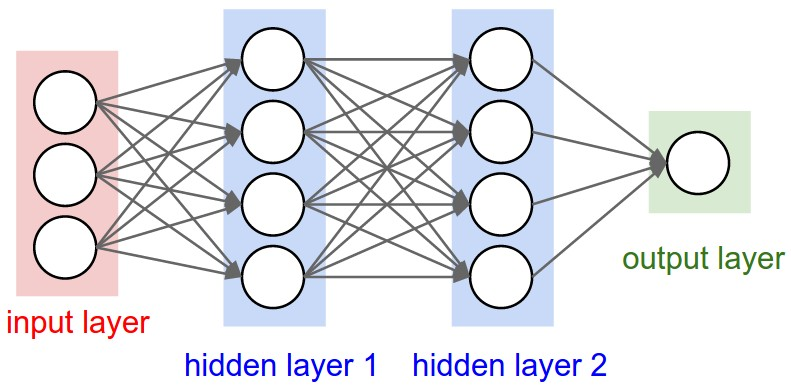
\includegraphics[width=0.7\textwidth]{Images/neural_net2.jpeg}
\captionof{figure}{\href{http://cs231n.github.io/neural-networks-1/}{[Ref: Neural Network]}}
}
\frame{\frametitle{Neural Network Outputs}
\begin{columns}
\begin{column}{0.48\textwidth}
\centering
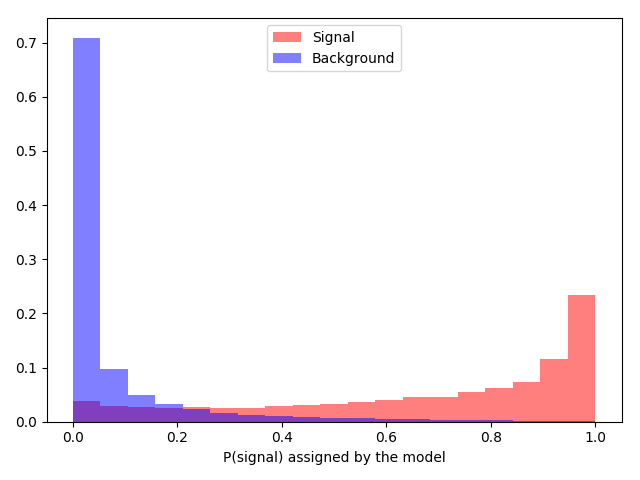
\includegraphics[width=1.0\textwidth]{Images/ejetsOuts/sigbkg.png} 
Neural Net Output
\end{column}
\begin{column}{0.48\textwidth}
\centering
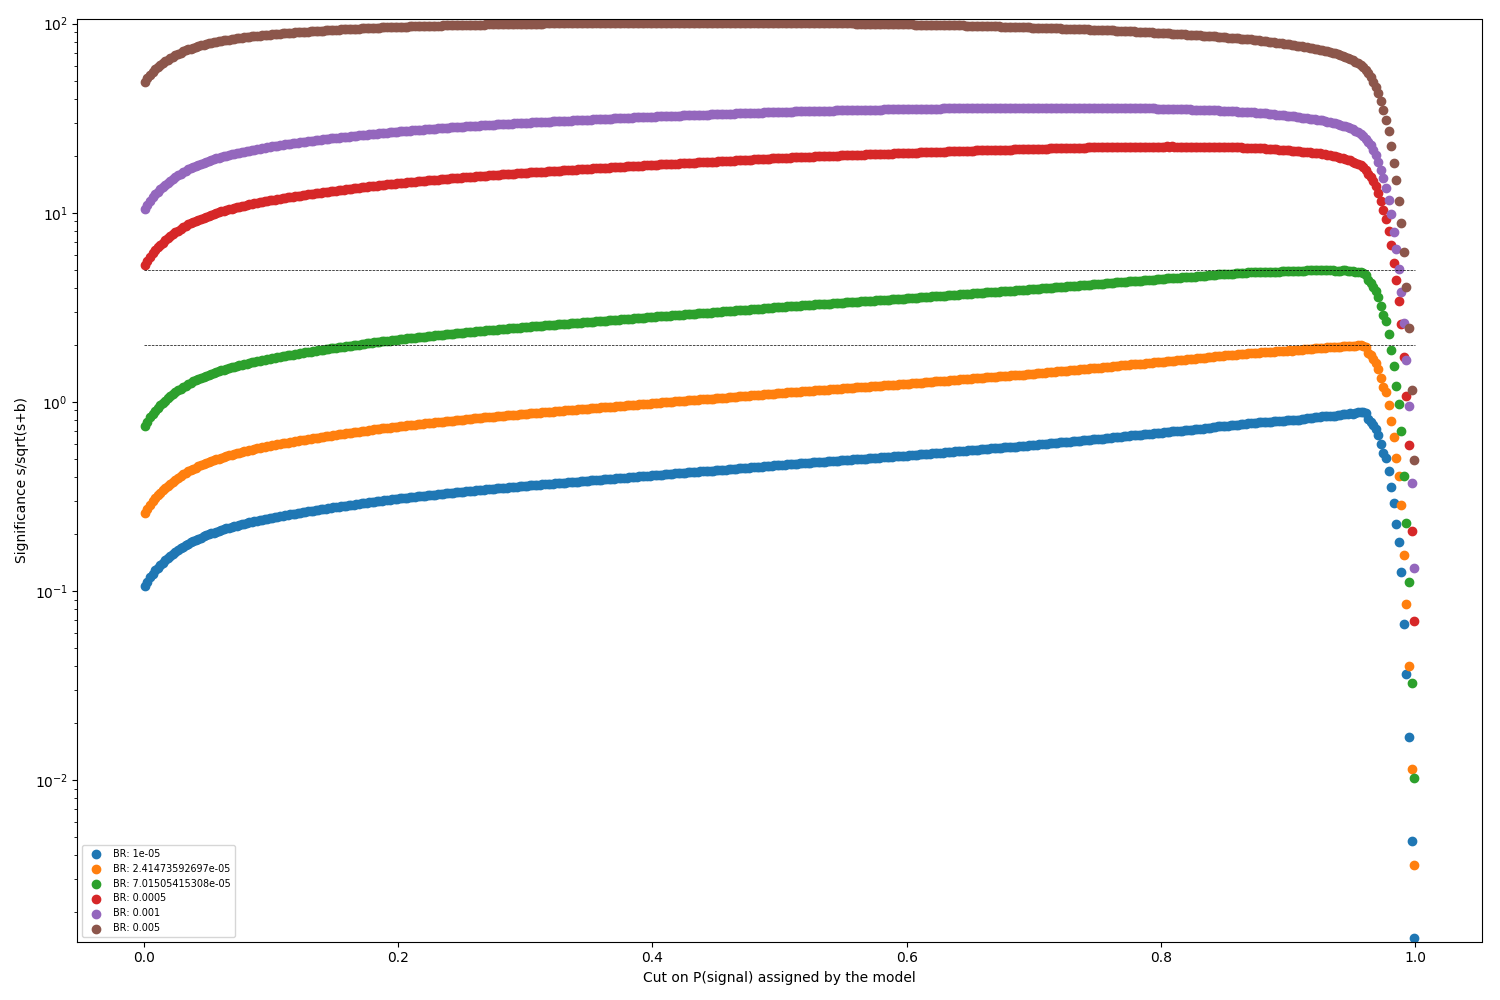
\includegraphics[width=1.0\textwidth]{Images/ejetsOuts/significance2.png} 
Significance
%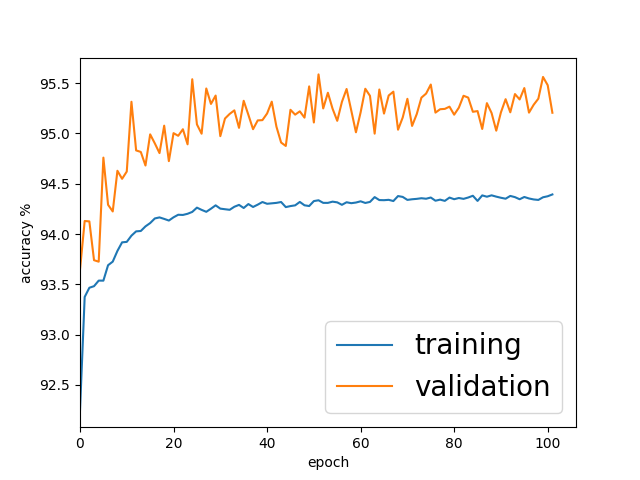
\includegraphics[width=0.85\textwidth]{Images/ejetsOuts/accuarcy.png} 
%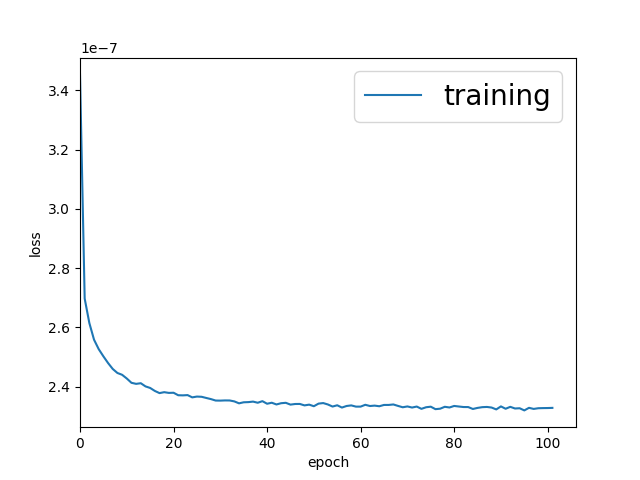
\includegraphics[width=0.85\textwidth]{Images/ejetsOuts/loss.png} 
\end{column}
\end{columns}
}


\frame{\frametitle{Neural Network Outputs}
\centering
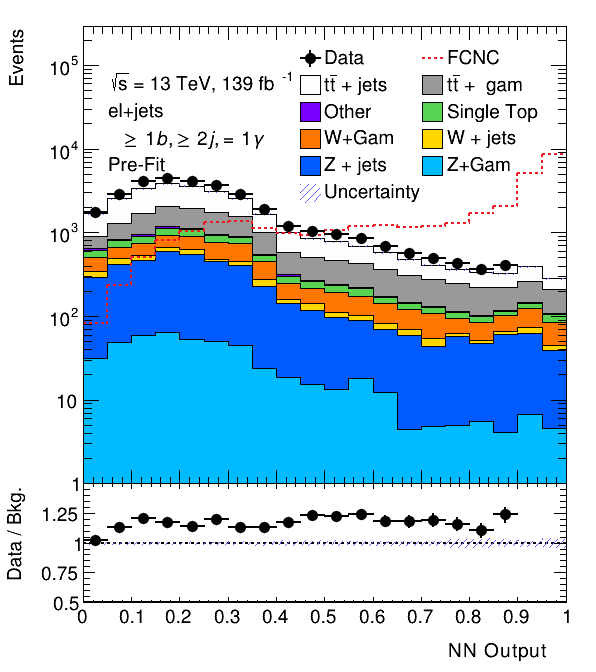
\includegraphics[width=.5\textwidth]{Images/PreSel_NNejet.png}\\
\begin{itemize}
\item Excellent signal/background separation achieved
\end{itemize}
}


%%%%%%%%%%%%%%%%%%%%%%%%%%%%%%%%%%%%%%%%%%%%%%%%%%%%%%%%%%%%%%%%%%
\section{Results and Conclusions}



\subsection{Work In Progress - Results}
\frame{\frametitle{Work In Progress - Results}
\begin{itemize}
\item Regions are used to compare background modeling behavior and data while not unblinding the signal region 
\end{itemize}
\begin{columns}
\begin{column}{0.35\textwidth}
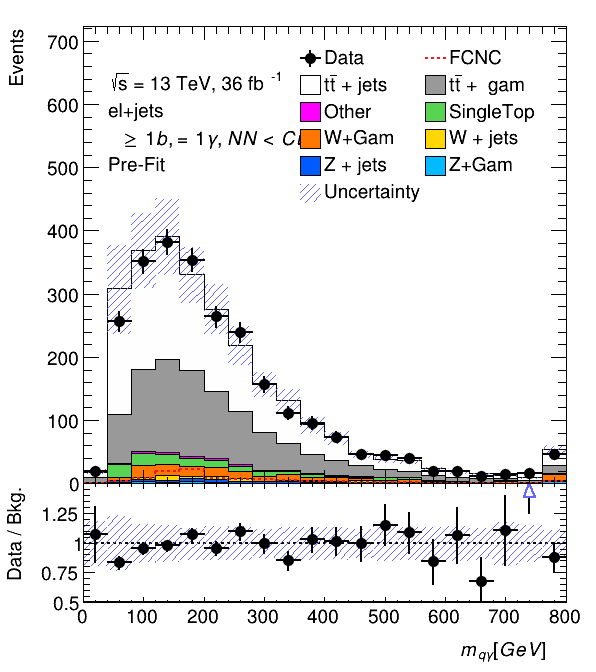
\includegraphics[width=.95\textwidth]{Images/SystwoSyst/Plots/VR2_mqph.png} \\
\end{column}
\begin{column}{0.35\textwidth}
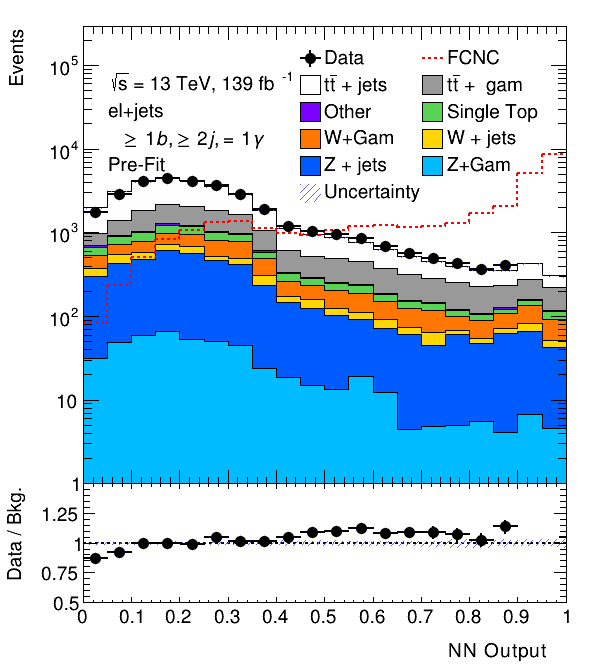
\includegraphics[width=.95\textwidth]{Images/FCNC_All_ejetsPreSelFitFactors/Plots/PreSel_NNejet.png}\\
\end{column}
\begin{column}{0.33\textwidth}
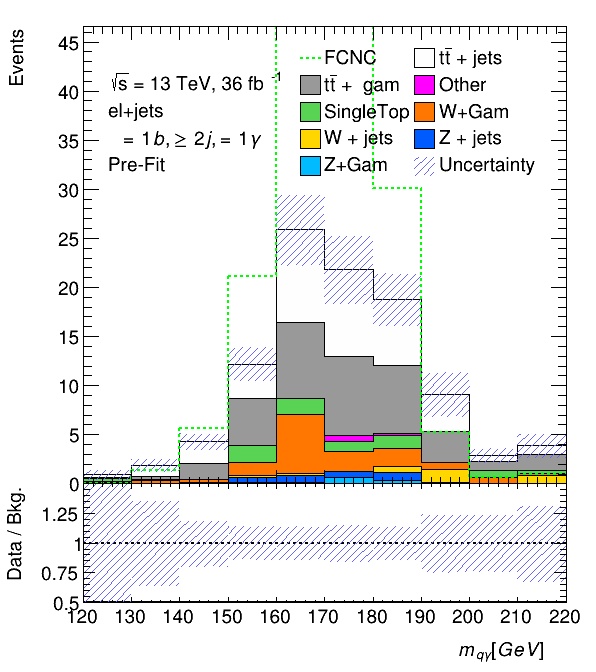
\includegraphics[width=.95\textwidth]{Images/SystwoSyst/Plots/SR_mqph.png} \\
\end{column}
\end{columns}
}




\frame{\frametitle{Conclusions}
\begin{itemize}
\item I have created model independent signal samples to search for flavor changing neutral current decays in top pair events
\item Developed and implemented a neural network for signal classification
\item Currently working to ensure well modeled backgrounds
\item Any excess in signal data events is a strong indication of physics beyond the Standard Model
\item Expected statistics only limit BR($t\rightarrow q \gamma) \leq 4 \times 10^{-5}$
\end{itemize}
\centering
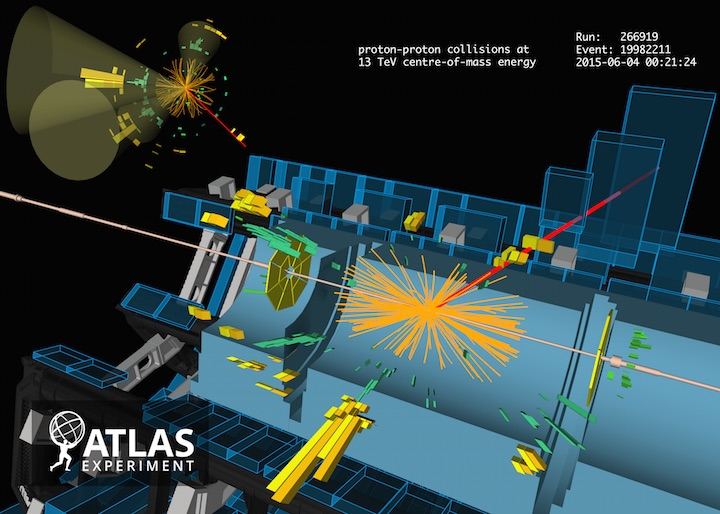
\includegraphics[width=.5\textwidth]{../../Thesis/ThesisImages/ttbarevent.jpg}
}



%%%%%%%%%%%%%%%%%%%%%%%%%%%%%%%%%%%%%%%%%%%%%%%%%%%%%%%%%%%%%%%%

\appendix
%\label{supplemental}
\section{Backup}
\subsection{Backup/Other Materials}
\frame{\frametitle{Backup}
\label{supplemental}
}

\subsection{Data Driven Backgrounds}
\frame{\frametitle{Data Driven Backgrounds}
\begin{itemize}
\item Various physics processes are known to be difficult to model, especially at the high energies and interaction rates of the LHC
\end{itemize}
\begin{columns}
\begin{column}{0.5\textwidth}
Before Scaling
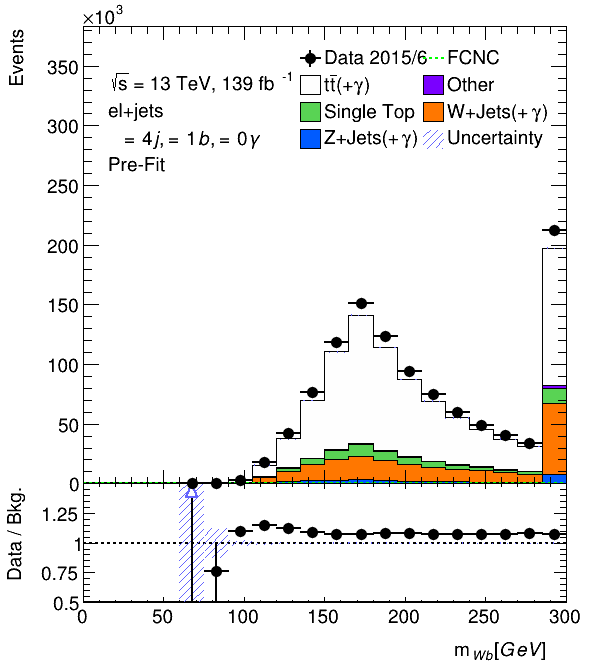
\includegraphics[width=.8\textwidth]{../../Thesis/ThesisImages/RegionPlots/AfterScaling/ControlRegions/HardCodedNormFactor/FCNC_All_ejets/Plots/VR3_SMtop.png} 
\end{column}
\begin{column}{0.5\textwidth}
After Scaling
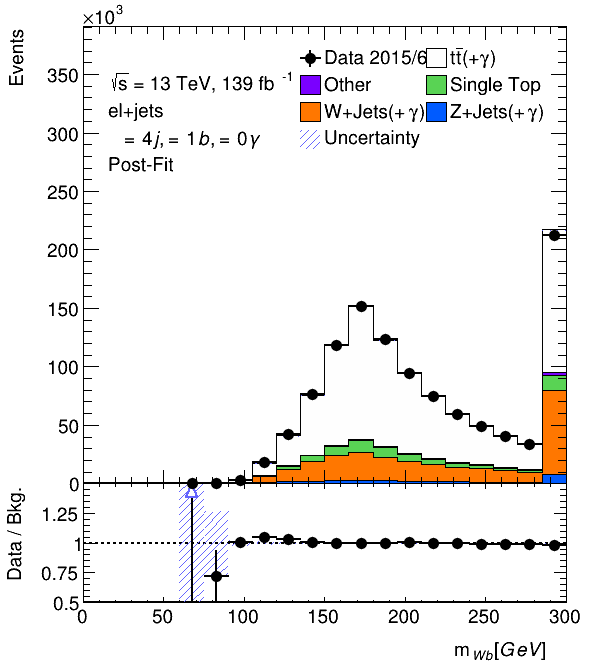
\includegraphics[width=.8\textwidth]{../../Thesis/ThesisImages/RegionPlots/AfterScaling/ControlRegions/HardCodedNormFactor/FCNC_All_ejets/Plots/VR3_SMtop_postFit.png}
\end{column}
\end{columns}
}
\frame{\frametitle{}

\begin{columns}
\begin{column}{0.02\textwidth}
\rotatebox{90}{$\mu$ channel  \qquad \qquad $e$ channel \qquad} 
%\rotatebox{90}{Muon Channel        } 
\end{column}
\begin{column}{0.48\textwidth}
\begin{itemize}
\item Converted Photons
%\item  MCee integral small range: 424,051.  - Vgam: 429789 - All 430225
%\item DATAee integral small range: 468,832
%\item MCeg integral small range: 110822     - Vgam: 115066 - All 152420
%\item DATAeg integral small range: 118198
\end{itemize}
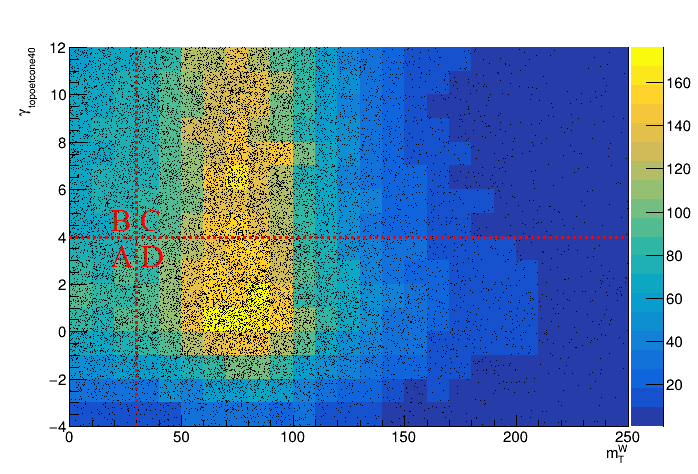
\includegraphics[width=.85\textwidth]{../../Thesis/ThesisImages/SearchStrategy/ABCD/ejetsConverted.png} \\
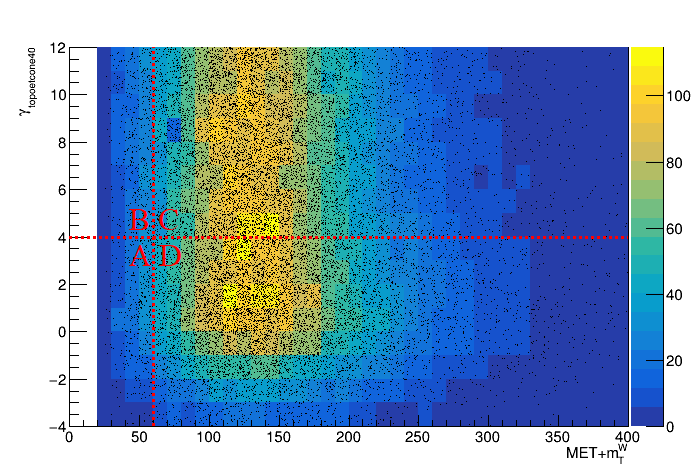
\includegraphics[width=.85\textwidth]{../../Thesis/ThesisImages/SearchStrategy/ABCD/mujetsConverted.png}
\end{column}
\begin{column}{0.48\textwidth}
\begin{itemize}
\item Unconverted Photons
\end{itemize}
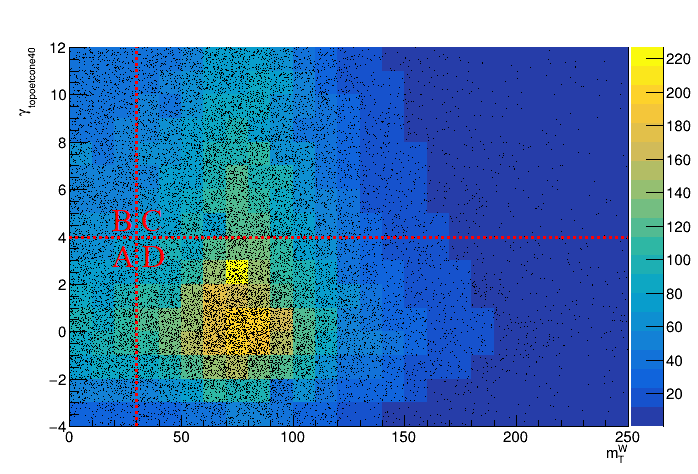
\includegraphics[width=.85\textwidth]{../../Thesis/ThesisImages/SearchStrategy/ABCD/ejetsUnconverted.png} \\
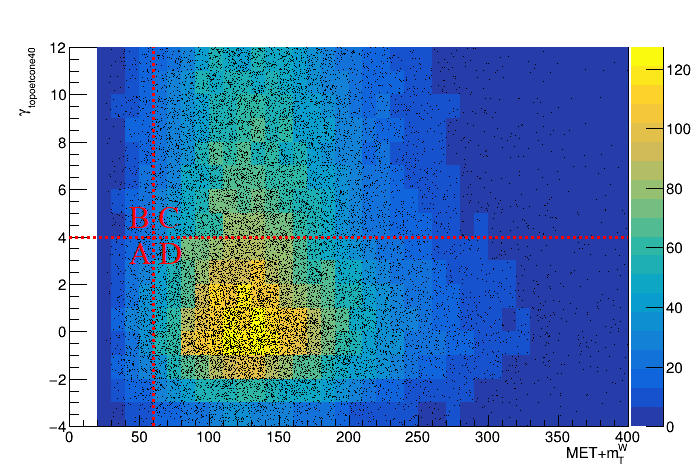
\includegraphics[width=.85\textwidth]{../../Thesis/ThesisImages/SearchStrategy/ABCD/mujetsUnconverted.png}
\end{column}
\end{columns}
\begin{table}[h]
\begin{center}
{\renewcommand{\arraystretch}{1.2}
\begin{tabular}{c|c|c}
\hline
Channel:     & Converted& Unconverted  \\  \hline 
Electron Channel  & $1.28\pm 0.34$     &   $1.99 \pm 0.52$	\\ 
Muon Channel        & $1.23 \pm 0.50$   &   $2.27 \pm 0.92$\\ \hline %Change Put in post fit values
\end{tabular}
}
\end{center}
\end{table}
}
\subsection{ATLAS Info}
\frame{\frametitle{Particles in ATLAS}
\centering
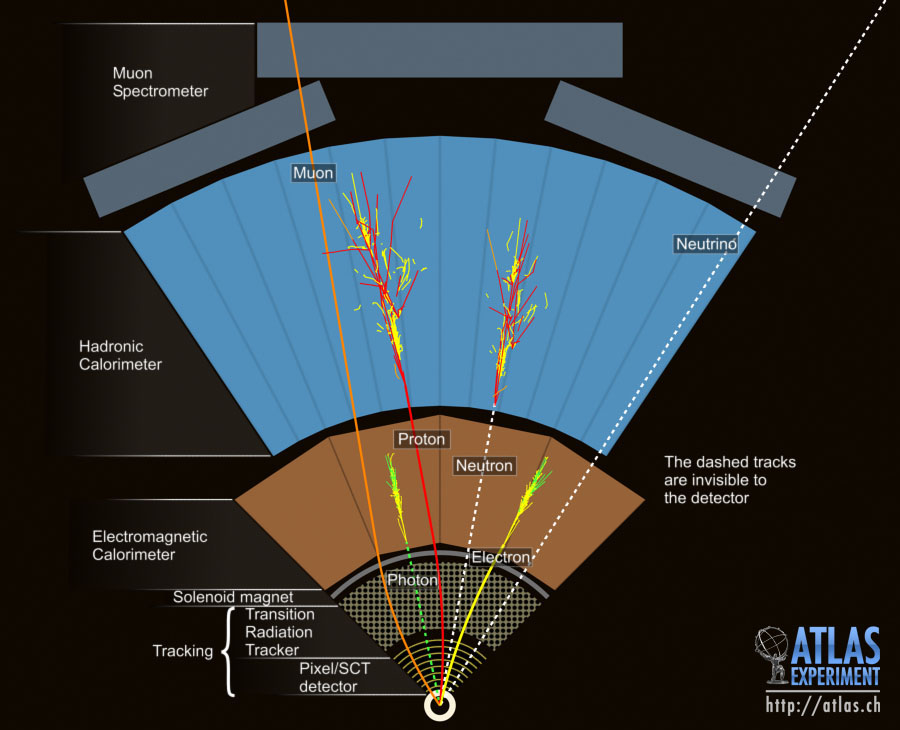
\includegraphics[width=.8\textwidth]{../../Thesis/ThesisImages/Simulation/ParticleInteractions.jpg}
}


\frame{\frametitle{Luminosity and Pile-up}
\centering
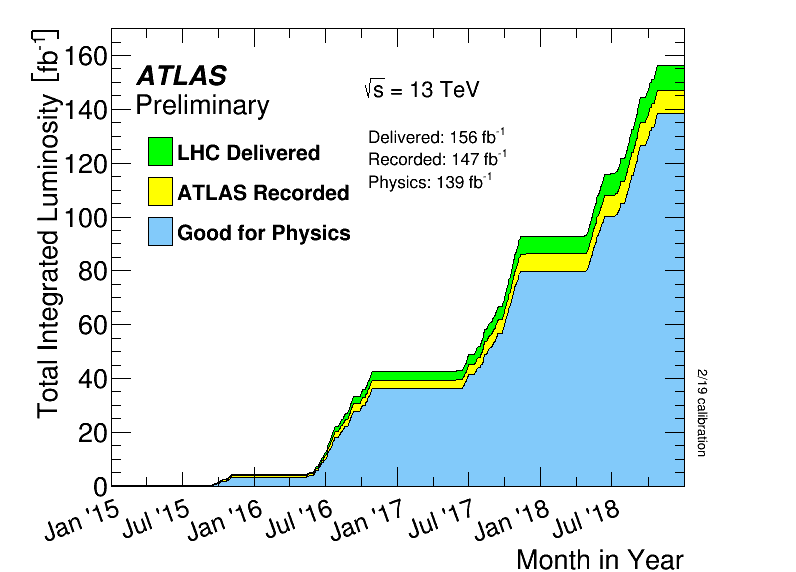
\includegraphics[width=.49\textwidth]{../../Thesis/ThesisImages/LHCImages/ATLASLumi.png}
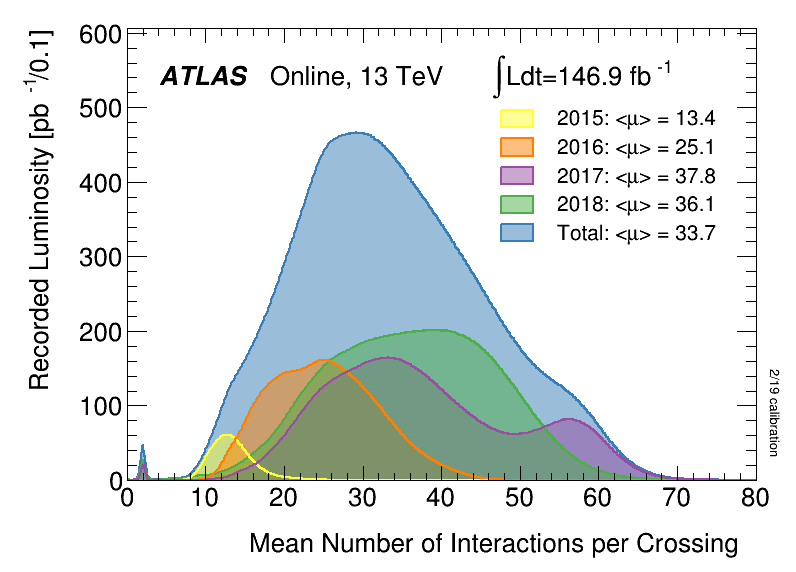
\includegraphics[width=.49\textwidth]{../../Thesis/ThesisImages/LHCImages/meanIntperCrossing.png}
}



\frame{\frametitle{FCNC Diagrams}
\centering
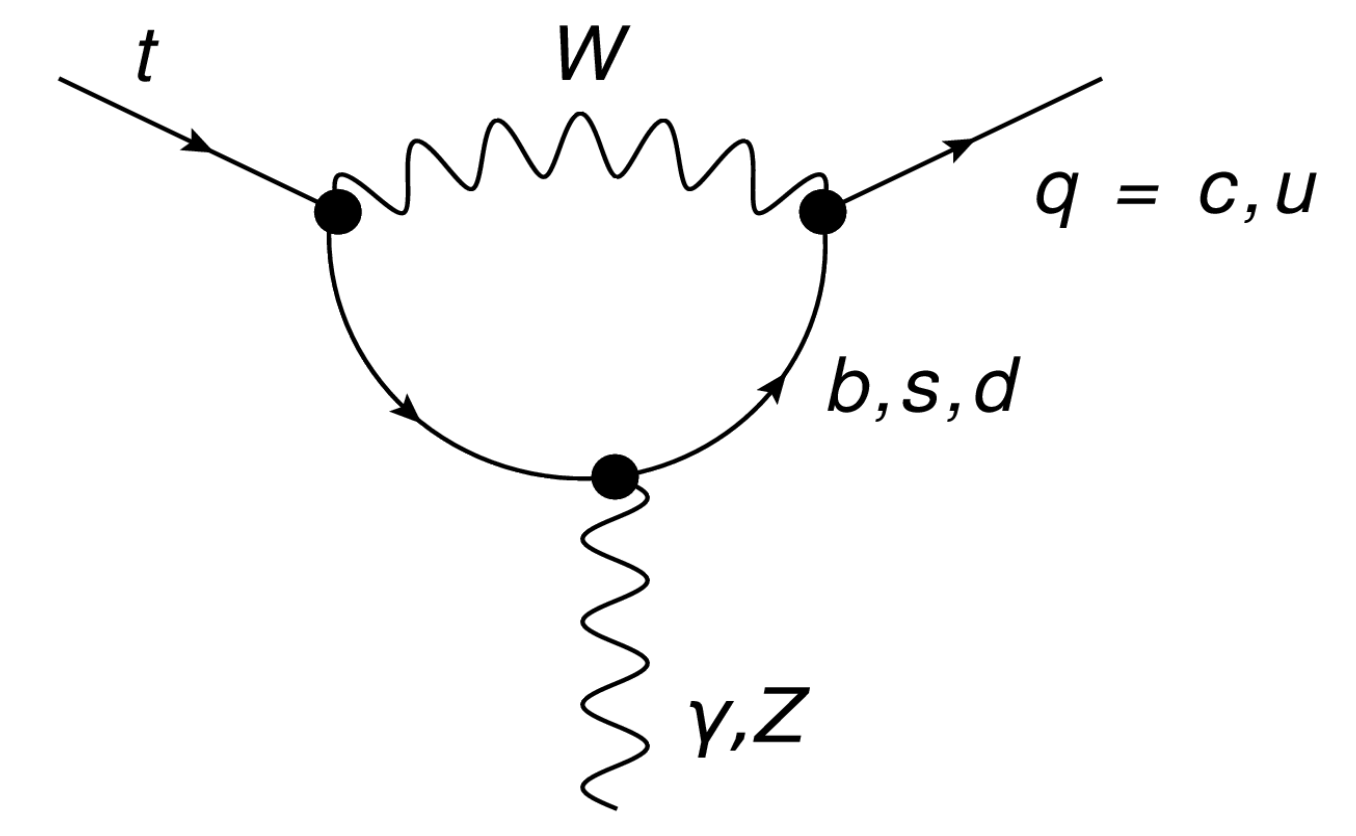
\includegraphics[width=.8\textwidth]{../../Thesis/ThesisImages/penguinFCNC.png}
}


%\frame{\frametitle{}
%}

\frame{\frametitle{Neural Network Model Inputs}
\centering
\scalebox{0.8}{ $\text{Separation} = \sum_{i}^{bins} \frac {n_{s i}-n_{b i}}{n_{s i}+n_{b i}}$}
\begin{columns}
\begin{column}{0.48\textwidth}
\centering
mu+jets channel\\
\scalebox{0.6}{\begin{tabular}{cc}
Variable & Separation \\
\hline
photon0iso & 41.18 \\
mqgam & 28.27 \\
photon0pt & 24.07 \\
mtSM & 11.60 \\
mlgam & 7.56 \\
deltaRjgam & 5.64 \\
deltaRbl & 4.42 \\
MWT & 3.34 \\
ST & 3.30 \\
nuchi2 & 3.12 \\
jet0pt & 2.81 \\
njets & 2.07 \\
smchi2 & 1.89 \\
wchi2 & 1.87 \\
jet0e & 1.52 \\
deltaRlgam & 1.17 \\
leptone & 0.87 \\
deltaRjb & 0.86 \\
met & 0.68 \\
bjet0pt & 0.52 \\
leptoniso & 0.27 \\
\end{tabular}
}
\end{column}
\begin{column}{0.48\textwidth}
\centering
e+jets channel \\
\scalebox{0.6}{\begin{tabular}{c c}
Variable & Separation\\
\hline
photon0pt & 23.14 \\
mqgam & 22.73 \\
photon0iso & 18.70 \\
mtSM & 11.02 \\
mlgam & 9.53 \\
deltaRbl & 5.00 \\
deltaRjgam & 4.60 \\
ST & 3.83 \\
MWT & 3.16 \\
jet0pt & 2.47 \\
njets & 1.70 \\
nuchi2 & 1.59 \\
deltaRlgam & 1.40 \\
wchi2 & 1.33 \\
smchi2 & 1.09 \\
deltaRjb & 0.88 \\
leptone & 0.85 \\
leptoniso & 0.56 \\
bjet0pt & 0.50 \\
met & 0.47 \\
\end{tabular}
}
\end{column}
\end{columns}
}


\subsection{ILC Info}
\frame{\frametitle{ILC ECAL1}
\begin{columns}
\begin{column}{0.5\textwidth}
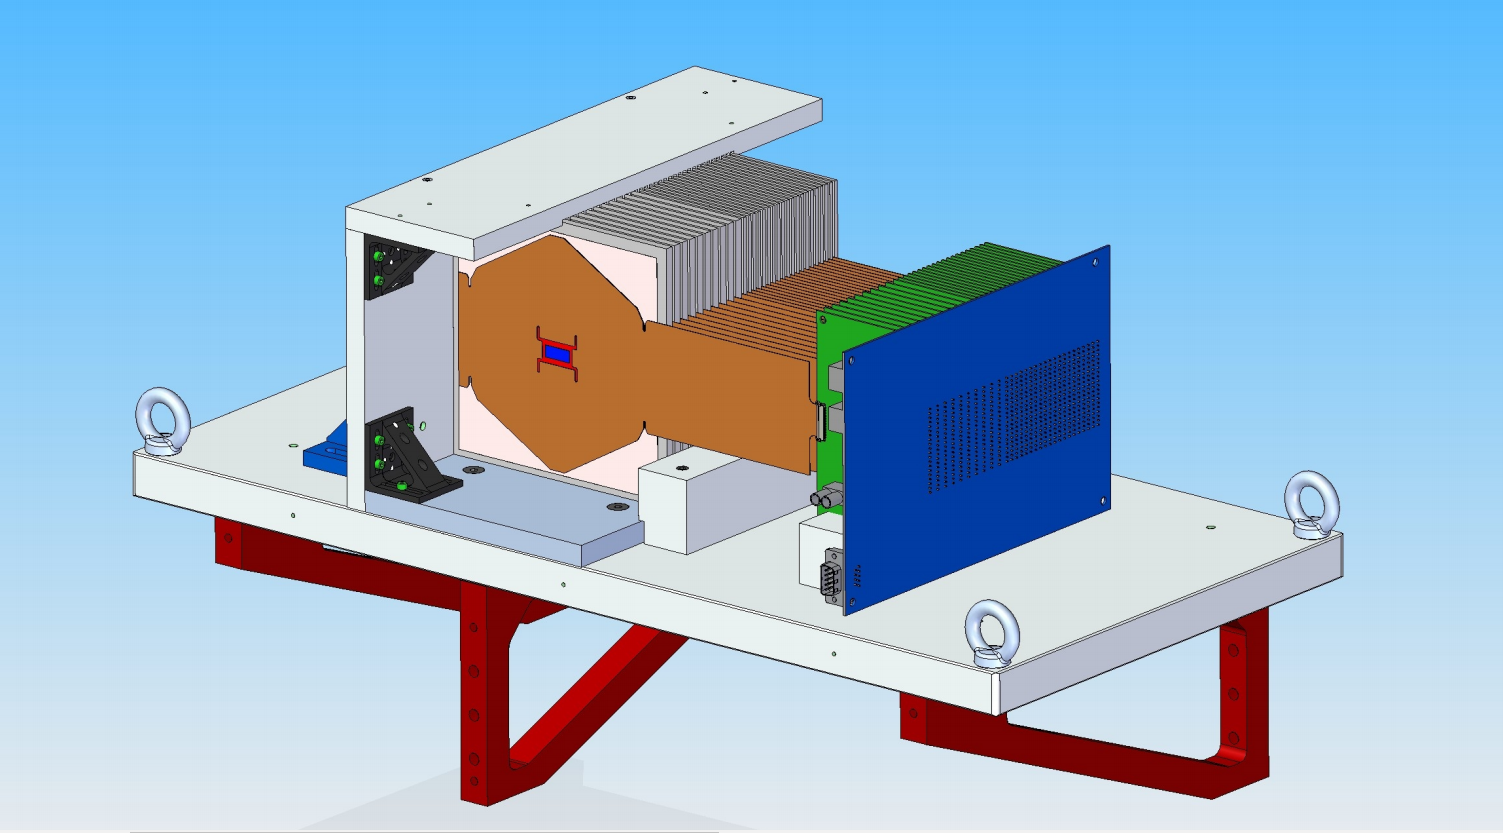
\includegraphics[width=.8\textwidth]{Images/EngDraw.png} \\
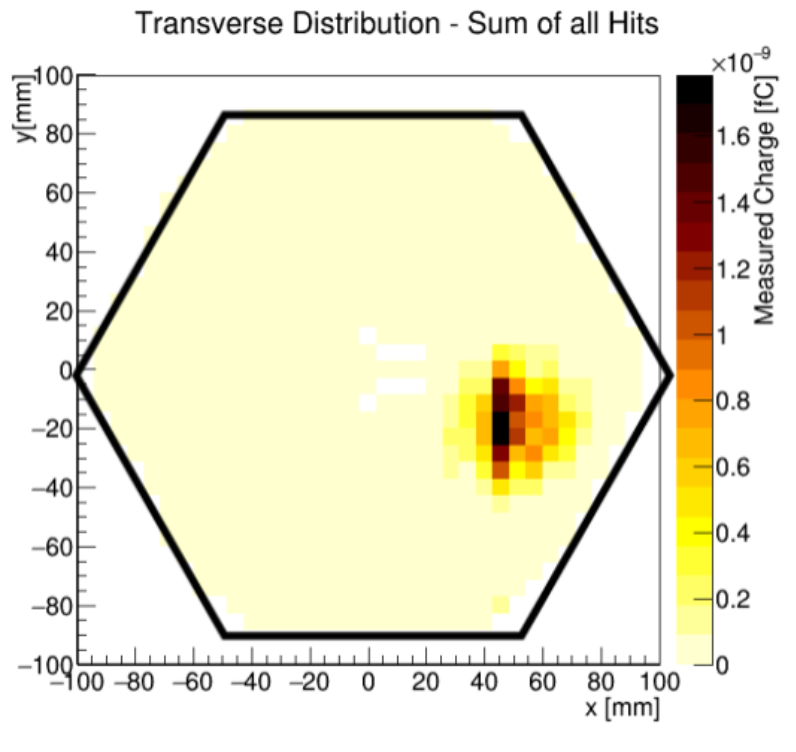
\includegraphics[width=.8\textwidth]{Images/SimulatedData.png}
\end{column}
\begin{column}{0.5\textwidth}
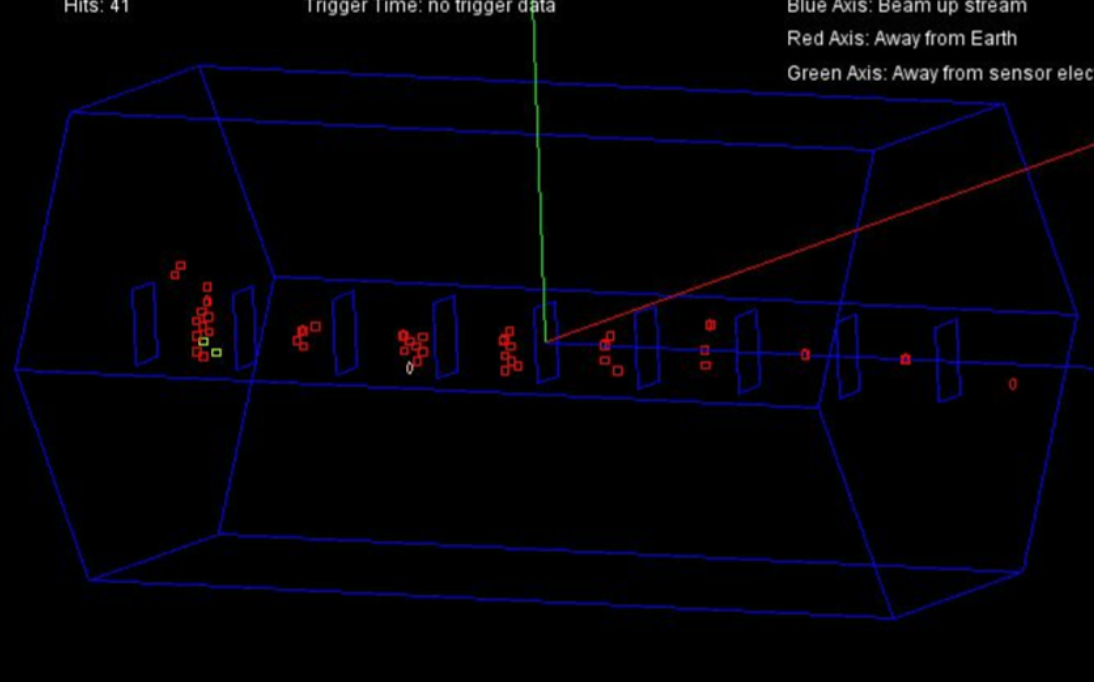
\includegraphics[width=\textwidth]{Images/DataRun.png} \\
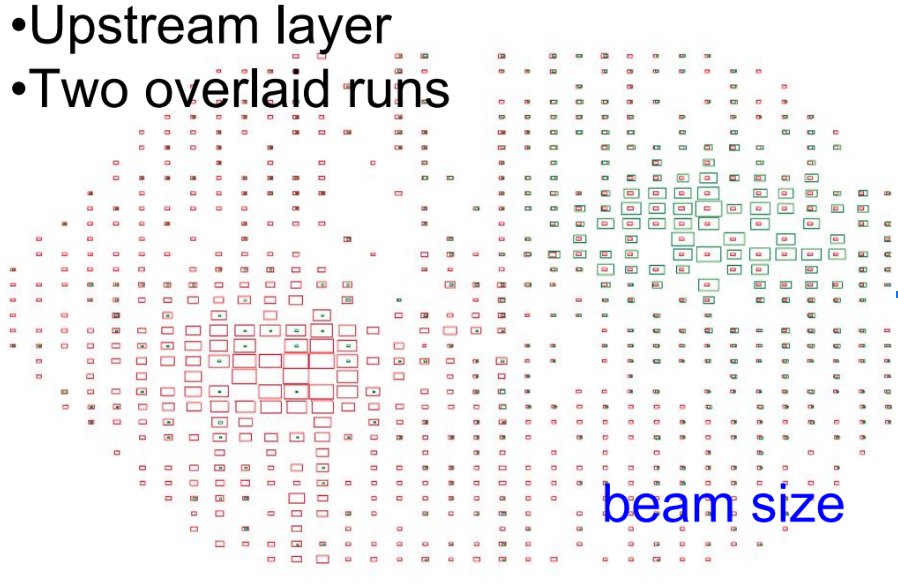
\includegraphics[width=\textwidth]{Images/Data.png}
\end{column}
\end{columns}
} 

\frame{\frametitle{ILC ECAL2}
\begin{columns}
\begin{column}{0.5\textwidth}
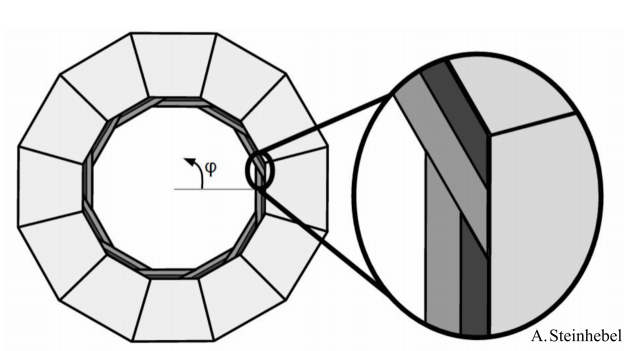
\includegraphics[width=.9\textwidth]{Images/ILCECal.png} \\
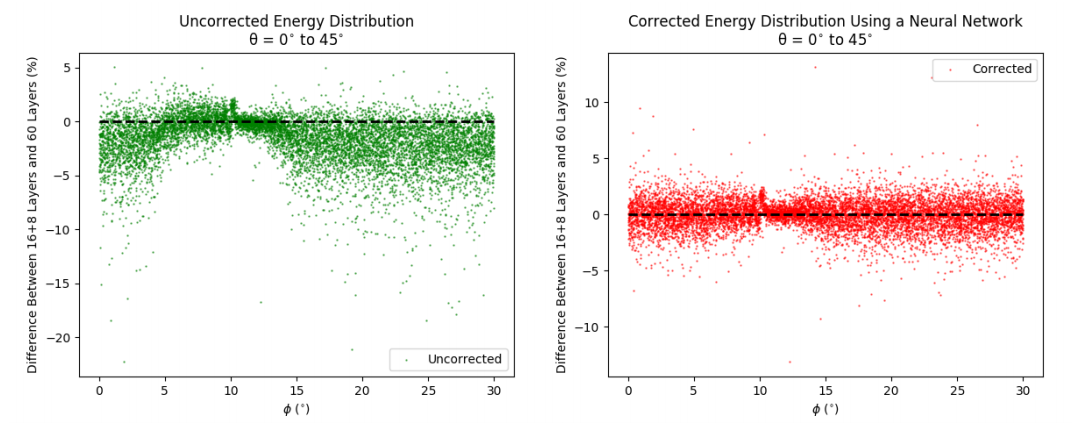
\includegraphics[width=1.\textwidth]{Images/NNCorrection.png}
\end{column}
\begin{column}{0.5\textwidth}
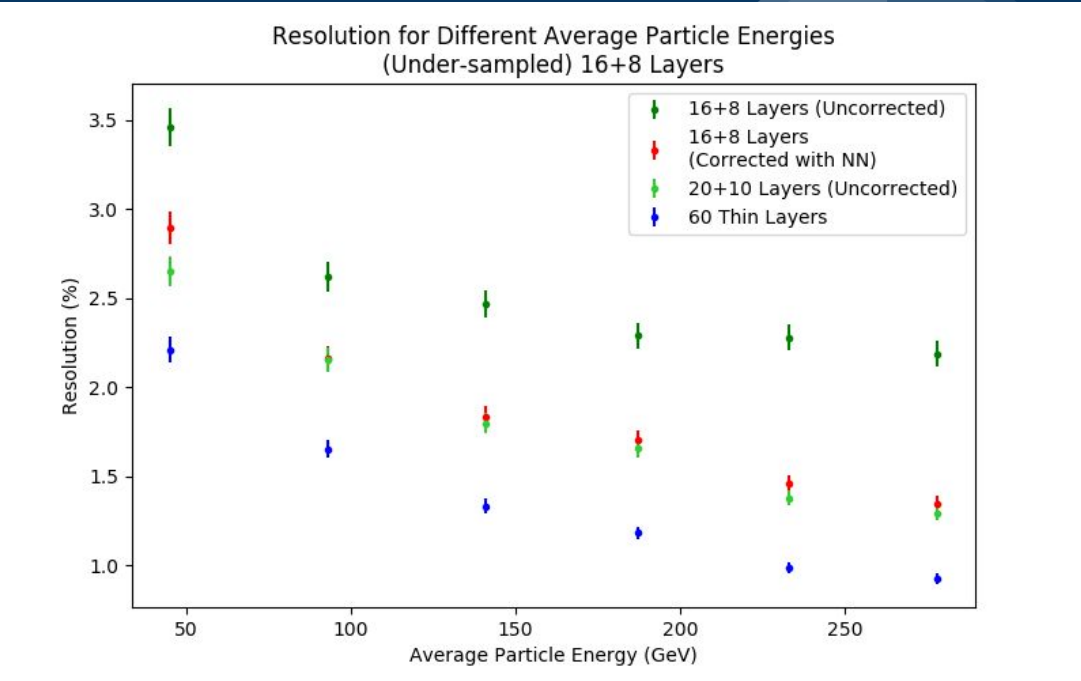
\includegraphics[width=.9\textwidth]{Images/ResoVEnergy.png} \\
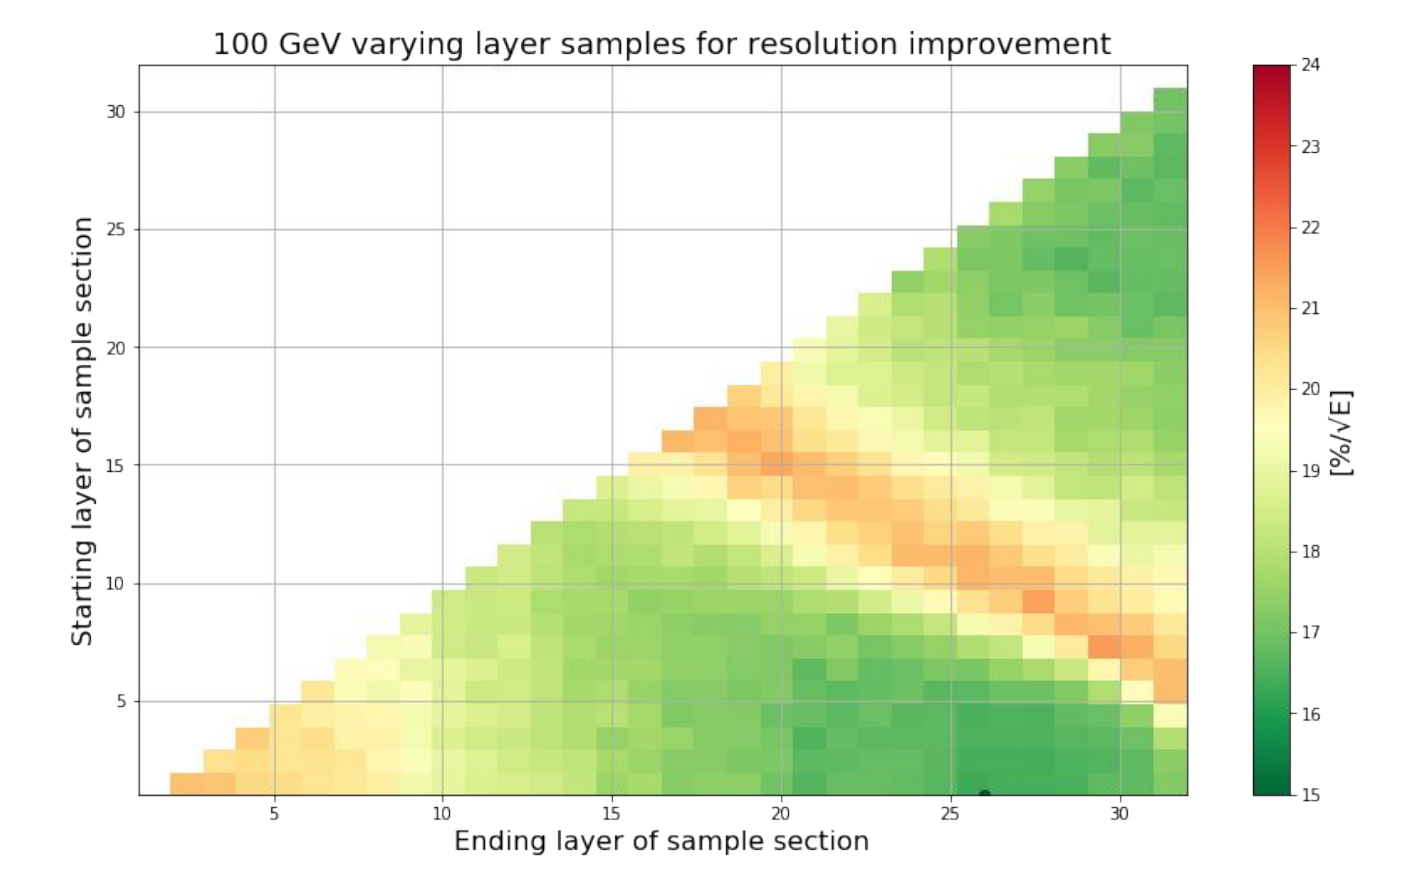
\includegraphics[width=.9\textwidth]{Images/ERes.png}
\end{column}
\end{columns}
}



%
%	\frame{\frametitle{Input Variables}
%	['photon0iso','photon0pt','mqgam','mlgam','mtSM','deltaRjgam','deltaRbl',\\
%	'MWT','ST','njets','wchi2','jet0pt','deltaRlgam','leptone','met','bjet0pt']
%	
%	
%	}

%\frame{\frametitle{Integrated Luminosity}
%\centering
%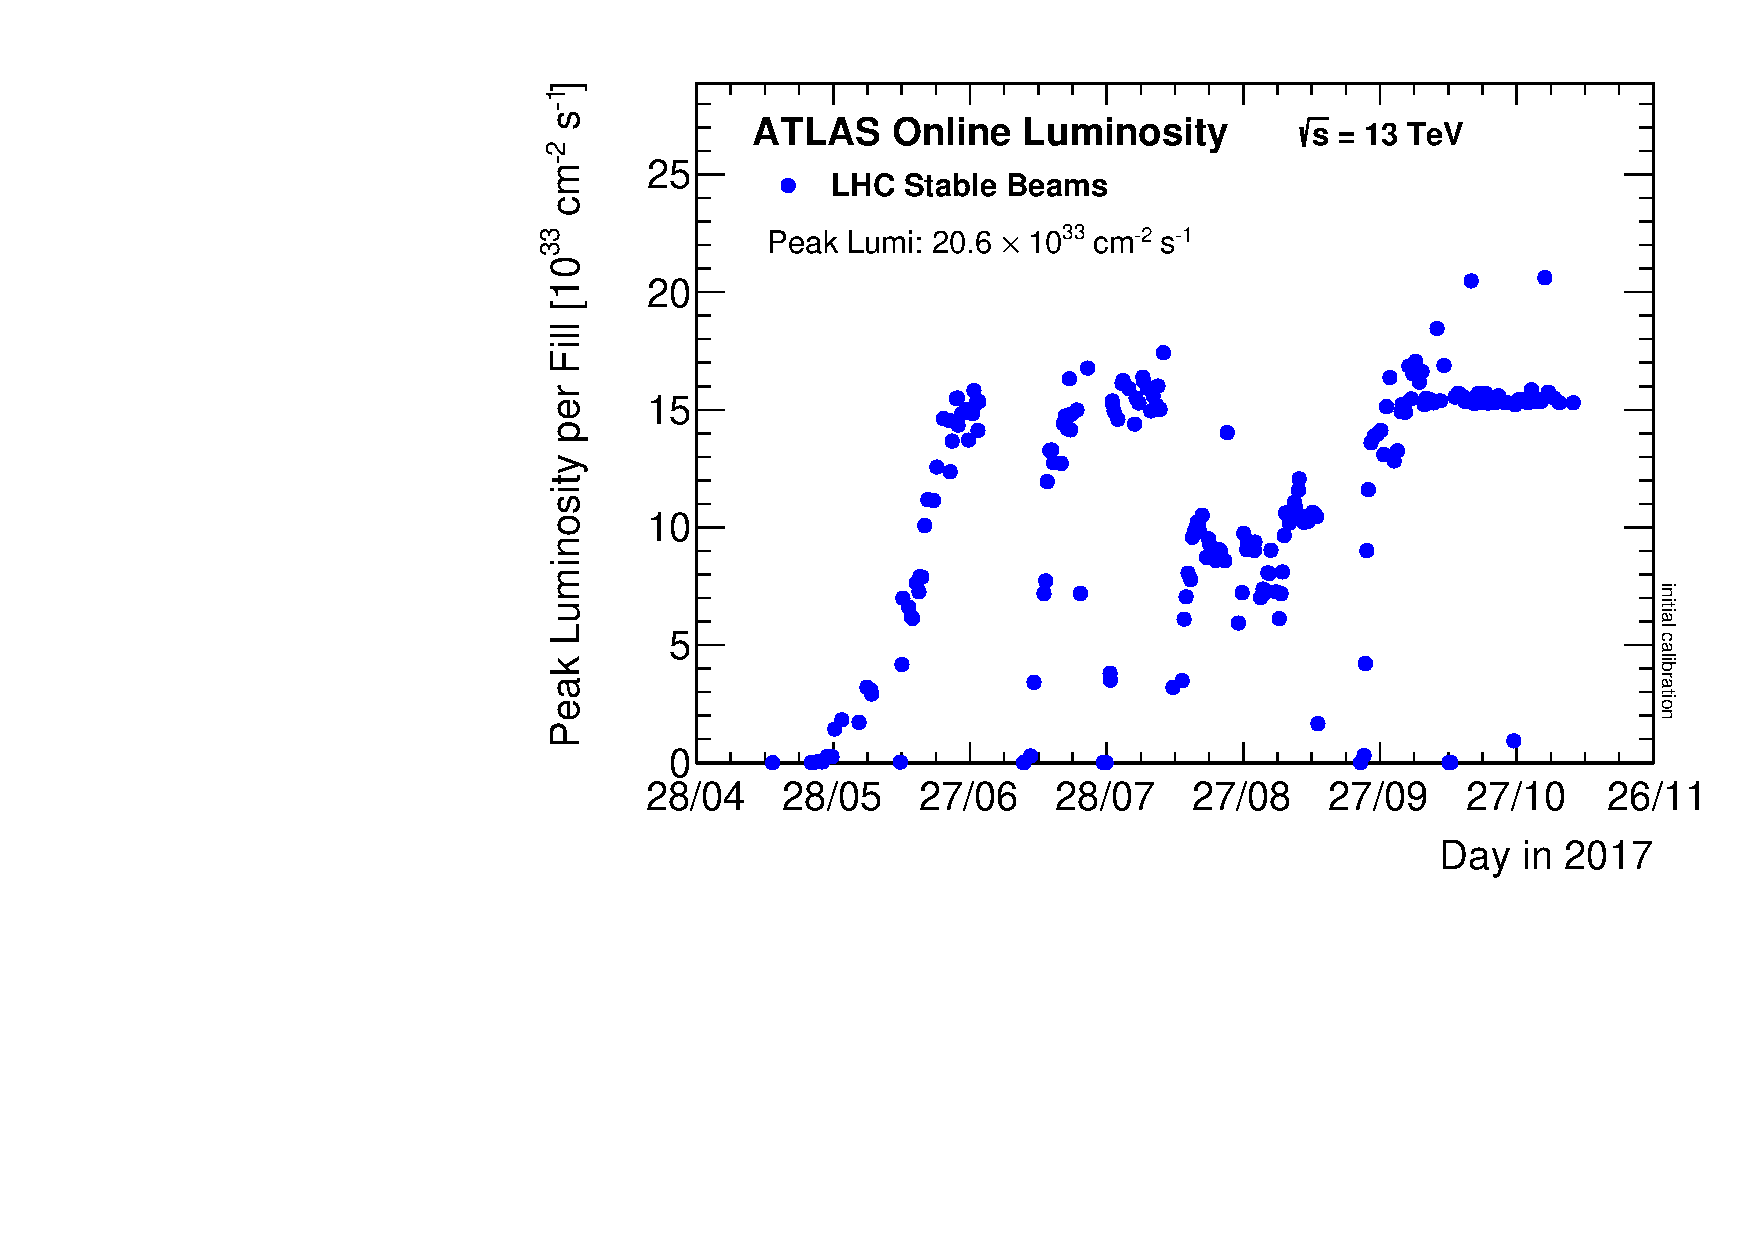
\includegraphics[width=1.\textwidth]{../../Thesis/ThesisImages/2017PeakLumiByFill.pdf}
%}
%\frame{\frametitle{A Couple BSM Diagrams}
%\centering
%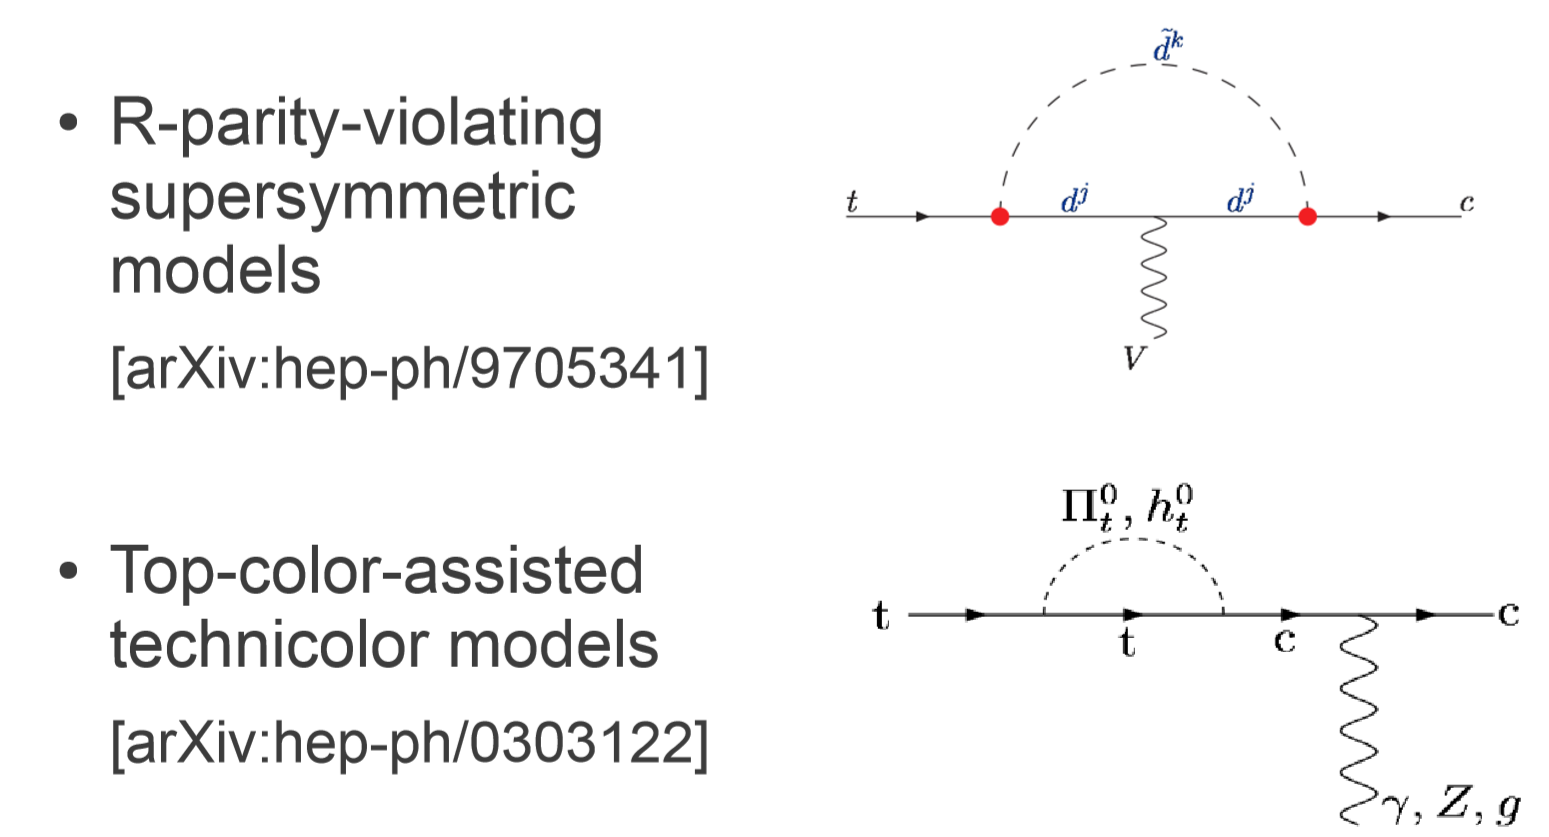
\includegraphics[width=1.\textwidth]{../../Thesis/ThesisImages/BSMDiagrams.png}
%}

%\frame{\frametitle{Jets/AntiKT}
%
%\[ d_{ij} = min(\frac{1}{p_{ti}^2},\frac{1}{p_{tj}^2}) \frac{\Delta_{ij}^2}{R^2}
%\]
%\[ d_{iB} = \frac{1}{p_{ti}^2}
%\]
%\[ \Delta_{ij}^2 = (\eta_i -\eta_j )^2 + (\phi_i - \phi_j )^2
%\]
%\begin{itemize}
%\item Find minimum of entire set of $\{ d_{ij},d_{iB} \}$
%\item If $d_{ij}$ is the minimum particles i,j are combined into one particle and removed from the list of particles
%\item If $d_{iB}$ is the minimum i is labelled as a final jet and removed from the list of particles
%\item Repeat until all particles are part of a jet with distance between jet axes $\Delta_{ij}$ is greater than R
%\end{itemize}
%}
%
%%\frame{\frametitle{B-tagging}
%%\centering
%%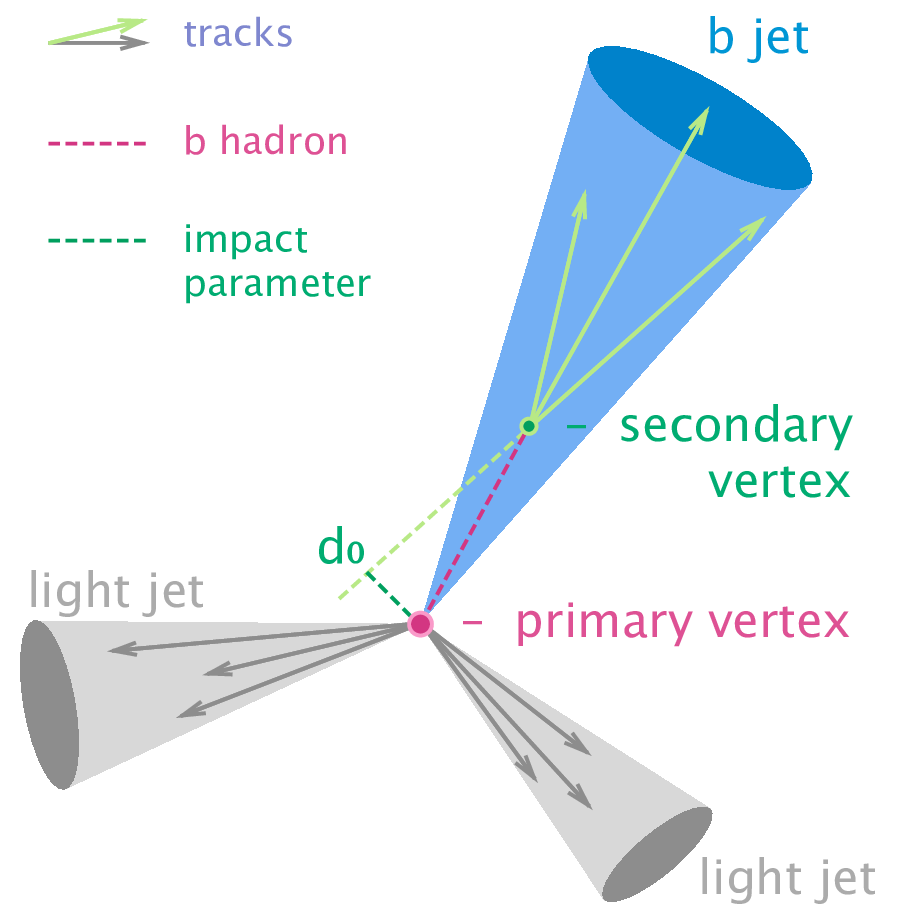
\includegraphics[height=.8\textheight]{../../Thesis/ThesisImages/SimulationNN/B-tagging_diagram.png}
%%}
%
%\frame{\frametitle{}
%\[ \mathcal{L}^{eff}_{tq\gamma} = - e \bar{c} \frac{i \sigma^{\mu\nu}q_{\nu}}{m_t}(\lambda^{L}_{ct}P_L + \lambda^{R}_{ct}P_{R}) t A_{\mu} +H.c.
%\]
%}

\end{document}

%36.070


%%% Neural Net Ref: http://cs231n.github.io/neural-networks-1/

% npart0=['photon0_iso','photon0_pt','m_qgam','m_lgam','m_tSM','deltaRjgam','deltaRbl','MWT','S_T','nbjets','njets','w_chi2','jet0_pt','nu_chi2','sm_chi2','deltaRlgam','lepton_e','met','lepton_iso','bjet0_pt']
%all vars

%npart = ['photon0_iso','photon0_pt','m_qgam','m_lgam','m_tSM','deltaRjgam','deltaRbl','MWT','S_T','njets','nbjets','w_chi2','jet0_pt','deltaRlgam','lepton_e','met','bjet0_pt']
%usual npart1

%npart1=['photon0_iso','photon0_pt','deltaRjgam','deltaRbl','MWT','S_T','njets','w_chi2','jet0_pt','deltaRlgam','lepton_e','met','bjet0_pt']
%minimal